\documentclass[conference]{IEEEtran}
\usepackage[utf8]{inputenc}
\usepackage[T1]{fontenc}
\usepackage[brazilian]{babel}
\usepackage{cite}
\usepackage{amsmath,amssymb,amsfonts}
\usepackage{graphicx}
\usepackage{textcomp}
\usepackage{xcolor}
\usepackage{url}
\usepackage{booktabs}
\usepackage{array}
\usepackage{tikz}
\usetikzlibrary{arrows.meta,positioning,fit,calc}
\usepackage[hidelinks]{hyperref}
% DOI clicável, impresso como "doi: 10.xxxx" (sem a URL inteira).
\newcommand{\doilink}[1]{doi: \href{https://doi.org/#1}{#1}}
\graphicspath{{../notebooks/figuras/}}

\begin{document}

\title{Estimativa de Risco de Lesões em Jogadores de Futebol a partir de Dados Públicos de Desempenho: uma Abordagem Baseada em Aprendizado de Máquina}

\author{
\IEEEauthorblockN{Eduardo Henrique Queiroz Almeida}
\IEEEauthorblockA{
\textit{Engenharia de Computação} \\
\textit{CEFET-MG}\\
Divinópolis, Minas Gerais, Brasil \\
eduardo.almeida@aluno.cefetmg.br}
\and
\IEEEauthorblockN{Sergio Henrique Quedas Ramos}
\IEEEauthorblockA{
\textit{Engenharia de Computação} \\
\textit{CEFET-MG}\\
Divinópolis, Minas Gerais, Brasil \\
sergio.ramos@aluno.cefetmg.br}
}

\maketitle

\begin{abstract}
Modelos que estimam o risco de lesão no futebol costumam depender de GPS e de dados internos dos clubes, aos quais pesquisadores de fora não têm acesso. Este trabalho verifica se dados públicos de partidas bastam para apontar quais jogadores têm mais risco de se lesionar nos $14$ dias seguintes a um jogo. Com dados do Transfermarkt, montamos uma base da Série~A do Brasileirão de 2022 a 2025, com $47{.}704$ partidas de $1{.}579$ jogadores e $1{.}212$ lesões. Antes de modelar, constatamos que o site passou a registrar cerca de três vezes mais lesões a partir de 2024, o que obriga a separar os anos na avaliação. Comparamos quatro modelos de aprendizado de máquina. O melhor deles, uma regressão logística treinada em 2024 e testada em 2025, formou com os $10\%$ de jogos de maior risco um grupo com o dobro da taxa média de lesões. Esse desempenho vem do histórico de lesões do jogador e do número de jogos que o clube tem pela frente. A carga de minutos jogados acrescentou pouco ou nada. O modelo serve para triagem e não tem valor de diagnóstico.
\end{abstract}

\begin{IEEEkeywords}
lesões esportivas, futebol, aprendizado de máquina, carga de jogo, dados públicos, Transfermarkt
\end{IEEEkeywords}

\section{Introdução}

O futebol profissional depende do atleta em campo. Uma lesão tira o jogador de partidas, reduz o rendimento do time e o valor de mercado do atleta e, em casos graves, encurta a carreira. Por muito tempo, prevenir lesões foi tarefa só de médicos e fisiologistas. Com o monitoramento de desempenho e o aprendizado de máquina (\textit{machine learning}, ML), parte dessa decisão passou a se apoiar em dados.

A maioria dos estudos mede a carga de treino com GPS, sensores e frequência cardíaca. Um resultado se repete: o risco sobe quando o atleta tem um pico de esforço recente, acima do que vinha sustentando \cite{gabbett2016}. Esses estudos, porém, usam dados internos dos clubes. Um pesquisador de fora não consegue repeti-los, e um clube sem esse equipamento não consegue aplicá-los.

Minutos jogados, sequência de jogos e histórico de lesões são públicos. Um texto técnico do setor propõe que essas informações bastariam para estimar o risco \cite{jaja2026}, mas não apresenta evidência. Este trabalho testa essa ideia no Campeonato Brasileiro Série~A, de 2022 a 2025, com dados do Transfermarkt. Para cada partida, calculamos atributos de carga de minutos, de calendário e de histórico de lesões, e comparamos quatro modelos de ML na tarefa de prever lesão nos $14$ dias seguintes. Também medimos quanto a fonte mudou a forma de registrar lesões ao longo dos anos, um problema que os estudos com Transfermarkt costumam ignorar. O resultado é uma pontuação de risco relativo, útil para priorizar atenção, sem valor de diagnóstico médico.

\section{Revisão da Literatura}

A ideia de carga mais usada vem de Gabbett \cite{gabbett2016}. Carga alta e constante pode até proteger o atleta preparado para ela; o risco aparece quando a carga da última semana dispara em relação à das semanas anteriores. Essa comparação virou um índice, a razão aguda:crônica (ACWR), que divide a carga da última semana pela média das quatro anteriores. Valores entre $0{,}8$ e $1{,}3$ são considerados seguros, e valores de $1{,}5$ ou mais se associam a mais lesões. Williams \textit{et al.}~\cite{williams2017} propuseram uma variante com médias móveis exponenciais (EWMA), que dão mais peso aos dias recentes. Em outra linha, uma revisão de Page \textit{et al.}~\cite{page2023} encontrou mais lesões em períodos com jogos muito próximos, com $4$ dias ou menos de intervalo.

A Tabela~\ref{tab:literatura} resume os estudos mais próximos deste. Os que usam GPS chegam a bons resultados, mas com um único clube, poucos atletas e dados que ninguém de fora possui \cite{rossi2018,saberisani2025,majumdar2024,huth2026}. Eles mostram também um padrão da tarefa: como a lesão é rara, os modelos capturam muitas lesões ao custo de muitos alarmes falsos. Majumdar \textit{et al.}~\cite{majumdar2024} chegam a $77\%$ das lesões detectadas, mas só $13\%$ dos alertas se confirmam. Huth \textit{et al.}~\cite{huth2026}, com GPS e uma lesão a cada $170$ observações, mostram quão modesto o resultado pode ser mesmo com dados ricos.

\begin{table*}[!t]
\caption{Estudos relacionados}
\label{tab:literatura}
\centering
\footnotesize
\begin{tabular}{>{\raggedright\arraybackslash}p{2.3cm} >{\raggedright\arraybackslash}p{3.4cm} >{\raggedright\arraybackslash}p{3.3cm} >{\raggedright\arraybackslash}p{2.6cm} >{\raggedright\arraybackslash}p{4.4cm}}
\toprule
Estudo & Dados & Amostra & Validação & Resultado principal \\
\midrule
Rossi \textit{et al.}~\cite{rossi2018} & GPS de treino & 1 clube, 26 jogadores, 1 temporada & dentro da temporada & 80\% das lesões detectadas; 50\% dos alertas corretos \\
Saberisani \textit{et al.}~\cite{saberisani2025} & GPS de treino e jogo & 1 clube iraniano, 25 jogadores, 1 temporada & dentro da temporada & AUC de 0,91 com o número de desacelerações \\
Majumdar \textit{et al.}~\cite{majumdar2024} & GPS, antropometria e carga & 1 clube inglês, 35 jogadores, 5 temporadas & temporal & 77\% das lesões detectadas; 13\% dos alertas corretos \\
Huth \textit{et al.}~\cite{huth2026} & GPS (futebol feminino) & 1 clube, 34 jogadoras, 4 temporadas & temporal & AUC de 0,74; AP de 0,04 com 0,58\% de positivos \\
Chang \textit{et al.}~\cite{chang2024} & públicos, agregados por temporada & Premier League, 532 jogadores, 1 temporada & aleatória & AUC de 0,54 a 0,70; clube foi o preditor mais forte \\
Everett \textit{et al.}~\cite{everett2024} & Transfermarkt e eventos da StatsBomb & Premier League, 2 temporadas & aleatória & ganho pequeno sobre uma regra simples \\
Tonizzo~\cite{tonizzo2025} & FBref e Transfermarkt & Serie A italiana, 100 jogadores, 3 temporadas & temporal & F1 de 0,24 com reamostragem e 0 sem ela \\
\bottomrule
\end{tabular}
\end{table*}

Os estudos com dados públicos deixam outras lacunas. Chang \textit{et al.}~\cite{chang2024} usam uma temporada, estatísticas somadas por temporada e divisão aleatória dos dados, o que mistura passado e futuro; o clube aparece como o preditor mais forte. Everett \textit{et al.}~\cite{everett2024} também dividem os dados ao acaso e usam, além dos minutos, eventos de jogo da StatsBomb. Tonizzo~\cite{tonizzo2025} conclui que faltam informações nas fontes públicas para um bom desempenho. A revisão de Majumdar \textit{et al.}~\cite{majumdar2022} aponta problemas que se repetem: cada estudo escolhe suas próprias medidas de carga, poucos tratam bem a raridade das lesões e quase nenhum valida o modelo em temporadas diferentes. Na revisão de Leckey \textit{et al.}~\cite{leckey2025}, Random Forest e XGBoost aparecem entre os melhores métodos, mas a regressão logística ainda venceu em 4 de 12 estudos.

Não encontramos estudo com o Brasileirão inteiro, várias temporadas e validação que respeite a ordem do tempo. Este trabalho procura responder a duas perguntas nesse cenário. Um modelo treinado só com dados do Transfermarkt consegue ordenar o risco de lesão melhor do que o acaso? E a carga de minutos acrescenta algo ao que o histórico de lesões e o calendário já informam?

\section{Materiais e Métodos}

A Figura~\ref{fig:fluxo} resume as etapas. Cada observação é uma partida da Série~A em que o jogador entrou em campo. O alvo vale $1$ se o jogador sofre uma lesão (excluídas doenças e afastamentos por cansaço) entre o dia seguinte ao jogo e $14$ dias depois, e $0$ caso contrário. Quando a lesão começa no próprio dia do jogo ($168$ casos), a linha sai da análise principal, porque o evento já aconteceu durante a observação. Como muitas lesões de jogo aparecem no site com a data do dia seguinte, repetimos a análise incluindo o dia do jogo.

\begin{figure*}[!t]
\centering
\begin{tikzpicture}[
  font=\footnotesize\sffamily,
  box/.style={draw, rounded corners=2pt, align=center, inner sep=3.5pt,
              text width=2.02cm, minimum height=1.12cm},
  arr/.style={-{Latex}, thick}
]
\node[box] (a) {1. Coleta\\Transfermarkt\\elenco, lesões,\\partidas};
\node[box, right=0.22cm of a] (b) {2. Limpeza\\e auditoria\\dos registros};
\node[box, right=0.22cm of b] (c) {3. Atributos\\carga, calendário,\\histórico; alvo\\em 14 dias};
\node[box, right=0.22cm of c] (d) {4. Preparação\\valores ausentes,\\escala};
\node[box, right=0.22cm of d] (e) {5. Divisão\\três cortes\\no tempo};
\node[box, right=0.22cm of e] (f) {6. Modelos\\RL, RF,\\XGBoost, MLP};
\node[box, right=0.22cm of f] (g) {7. Avaliação\\métricas, ablação,\\interpretação};
\draw[arr] (a) -- (b);
\draw[arr] (b) -- (c);
\draw[arr] (c) -- (d);
\draw[arr] (d) -- (e);
\draw[arr] (e) -- (f);
\draw[arr] (f) -- (g);
\end{tikzpicture}
\caption{Etapas do estudo, da coleta pública à comparação dos modelos. Os atributos usam apenas informação disponível antes da partida.}
\label{fig:fluxo}
\end{figure*}

\subsection{Base de dados}

Não há fonte oficial de lesões no futebol brasileiro. Usamos o Transfermarkt\footnote{\url{https://www.transfermarkt.com.br/}}, site que registra elencos, lesões e partidas e já foi usado em estudos semelhantes. Para todos os clubes da Série~A de 2022 a 2025 (20 por ano, 28 diferentes no período), coletamos o elenco de cada temporada, o histórico de lesões de cada jogador (tipo, início, fim e jogos perdidos) e o registro de cada partida (data, competição, minutos jogados e se o jogador foi titular). A coleta respeitou um intervalo de $2{,}5$ a $5$ segundos entre acessos ao site, e os dados brutos não são redistribuídos.

A base final tem $47{.}704$ observações de $1{.}579$ jogadores, de abril de 2022 a dezembro de 2025, com $2{.}367$ casos positivos ($4{,}96\%$). A Tabela~\ref{tab:base} mostra os números por ano. Das lesões registradas no período, as mais comuns foram de coxa ($23{,}6\%$), joelho ($15{,}8\%$), musculares sem local definido ($15{,}4\%$) e tornozelo ($8{,}4\%$).

\begin{table}[!t]
\caption{Observações por ano (partidas da Série~A em que o jogador atuou)}
\label{tab:base}
\centering
\begin{tabular}{lrrrrr}
\toprule
Ano & Partidas & Jogadores & Positivos & Taxa (\%) & Lesões \\
\midrule
2022 & 11{.}929 & 748 & 308 & 2{,}58 & 150 \\
2023 & 11{.}926 & 739 & 233 & 1{,}95 & 121 \\
2024 & 11{.}928 & 709 & 828 & 6{,}94 & 416 \\
2025 & 11{.}921 & 736 & 998 & 8{,}37 & 525 \\
\midrule
Total & 47{.}704 & 1{.}579 & 2{.}367 & 4{,}96 & 1{.}212 \\
\bottomrule
\end{tabular}
\end{table}

\subsection{Auditoria dos registros}
\label{sec:auditoria}

Antes de modelar, verificamos a qualidade do alvo. Três pontos se destacaram.

Primeiro, uma mesma lesão gera vários casos positivos. Um jogador que atua a cada três ou quatro dias tem duas ou três partidas dentro da janela de $14$ dias anterior à lesão. Por isso os $2{.}367$ positivos correspondem a apenas $1{.}212$ lesões diferentes (última coluna da Tabela~\ref{tab:base}). Esse é o tamanho real da amostra, e ele é pequeno: os anos de 2022 e 2023 somam só $271$ lesões.

Segundo, $55\%$ das lesões começam no dia do jogo ou no dia seguinte. A lesão sofrida em campo é o caso mais comum, o que justifica a análise que inclui o dia do jogo.

Terceiro, e mais importante, a taxa de lesões triplica a partir de 2024 (Tabela~\ref{tab:base}). Investigamos se isso seria um aumento real. O número de partidas por ano é estável, e o salto aparece também nas lesões graves, de $28$ dias ou mais de afastamento (Figura~\ref{fig:deriva}). Ao mesmo tempo, o site passou a registrar o dobro de lesões e a descrevê-las com mais detalhe. O aumento varia muito entre clubes, de $1{,}1$ a $13$ vezes, e a ordem dos clubes com mais lesões muda de um ano para o outro. A explicação mais provável é que o Transfermarkt passou a registrar lesões de forma mais completa, e mais em alguns clubes do que em outros. Essa mudança afeta também o histórico dos jogadores: a parcela de observações sem nenhuma lesão anterior registrada cai de $54\%$ em 2022--23 para $19\%$ em 2025. Por isso avaliamos os modelos separando anos com padrões de registro diferentes.

\begin{figure}[!t]
\centering
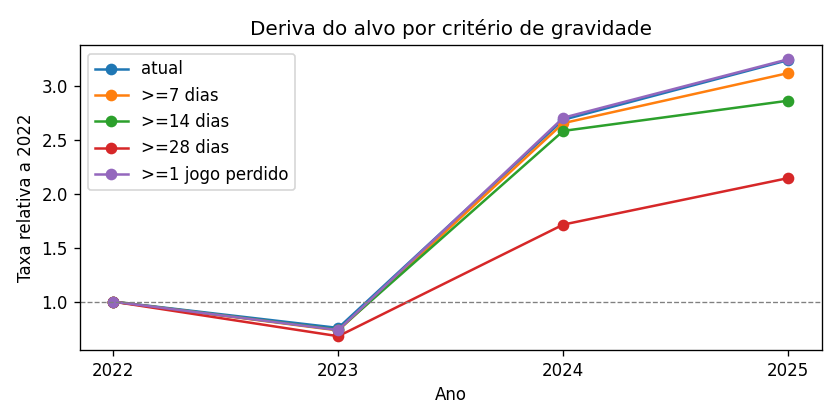
\includegraphics[width=\columnwidth]{04_deriva_por_gravidade.png}
\caption{Taxa de lesão por ano, relativa a 2022, considerando todas as lesões, só as com afastamento mínimo de 7, 14 e 28 dias e só as com pelo menos um jogo perdido. O salto de 2024--25 aparece em todos os casos.}
\label{fig:deriva}
\end{figure}

\subsection{Atributos}
\label{sec:prep}

Os atributos ficam em quatro grupos (Tabela~\ref{tab:feat}) e usam só informação anterior à partida. A carga considera todas as competições que o jogador disputou, e não só a Série~A: sem isso, quem jogou pela Copa na quarta-feira pareceria descansado no sábado.

\begin{table}[!t]
\caption{Atributos usados pelos modelos}
\label{tab:feat}
\centering
\begin{tabular}{>{\raggedright\arraybackslash}p{0.2\columnwidth} >{\raggedright\arraybackslash}p{0.7\columnwidth}}
\toprule
Grupo & Atributos \\
\midrule
Perfil & idade, titular, posição \\
Histórico & número de lesões (na carreira e em 12 meses), tempo desde a última lesão, duração da última lesão, tempo e jogos desde o retorno \\
Calendário & dias desde o último jogo, jogos nos últimos 30 dias, jogos do clube nos próximos 14 dias \\
Carga & minutos nos últimos 7 e 28 dias, ACWR, médias móveis exponenciais e sua razão \\
\bottomrule
\end{tabular}
\end{table}

A carga recente soma os minutos dos últimos $7$ dias, e a carga de base é a média semanal dos últimos $28$. A ACWR é a razão entre as duas. Testamos também a versão que separa as duas janelas, mas ela ordena os jogadores exatamente como a original e foi descartada. As médias móveis exponenciais seguem Williams \textit{et al.}~\cite{williams2017}.

O número de jogos do clube nos $14$ dias seguintes olha para o futuro, mas usa só a tabela de jogos, que é pública e conhecida antes da partida. Conferimos que o valor é o mesmo para quase todos os jogadores do elenco em cada jogo ($99{,}4\%$), então ele não traz informação individual sobre quem vai se lesionar.

O retorno de uma lesão é medido pela primeira partida que o jogador disputou depois dela, porque a data de fim registrada no site às vezes está errada. O clube ficou fora dos atributos: incluí-lo faria o modelo aprender o padrão de registro de cada clube, e não o risco do jogador.

Alguns atributos não existem para todas as observações, como o tempo desde a última lesão para quem nunca se lesionou. Nesses casos usamos um valor-limite e um indicador de ausência. Todas as transformações que dependem dos dados foram calculadas só com os dados de treino.

\subsection{Modelos}

Comparamos quatro modelos comuns nessa tarefa. A regressão logística é o modelo mais simples e serve de referência. O Random Forest e o XGBoost combinam muitas árvores de decisão e conseguem captar combinações entre atributos. O \textit{multilayer perceptron} (MLP) é uma rede neural pequena. Para cada modelo testamos poucas configurações (Tabela~\ref{tab:hiper}), escolhidas por validação cruzada dentro do treino, sem deixar partidas do mesmo jogador em treino e validação ao mesmo tempo. A rede neural foi treinada com $10$ inicializações diferentes, e usamos a média das previsões.

\begin{table}[!t]
\caption{Configurações testadas em cada modelo}
\label{tab:hiper}
\centering
\footnotesize
\begin{tabular}{>{\raggedright\arraybackslash}p{0.24\columnwidth} >{\raggedright\arraybackslash}p{0.66\columnwidth}}
\toprule
Modelo & Opções \\
\midrule
Reg. logística & regularização $C \in \{0{,}01;\ 0{,}1;\ 1\}$; com e sem peso de classe \\
Random Forest & 400 árvores; folha mínima de 25 ou 100; fração de atributos $\sqrt{p}$ ou 0,5 \\
XGBoost & 300 árvores; profundidade 2 a 4; peso mínimo por folha 5 ou 20; com e sem peso de classe \\
MLP & camadas de 32 e 16 neurônios; regularização $\alpha \in \{10^{-3};\ 10^{-2};\ 10^{-1}\}$ \\
\bottomrule
\end{tabular}
\end{table}

A Tabela~\ref{tab:escolhidas} mostra a configuração que venceu a validação cruzada em cada corte.

\begin{table}[!t]
\caption{Configuração escolhida pela validação cruzada em cada corte}
\label{tab:escolhidas}
\centering
\footnotesize
\setlength{\tabcolsep}{3pt}
\begin{tabular}{>{\raggedright\arraybackslash}p{0.2\columnwidth} >{\raggedright\arraybackslash}p{0.235\columnwidth} >{\raggedright\arraybackslash}p{0.235\columnwidth} >{\raggedright\arraybackslash}p{0.235\columnwidth}}
\toprule
Modelo & Corte A & Corte B & Corte C \\
\midrule
Reg. logística & $C = 0{,}01$, sem peso & $C = 1$, com peso & $C = 0{,}1$, com peso \\
Random Forest & folha 100, $\sqrt{p}$ & folha 100, 0,5 & folha 100, $\sqrt{p}$ \\
XGBoost & prof.~2, peso mín. 20, sem peso & prof.~2, peso mín. 5, sem peso & prof.~2, peso mín. 5, sem peso \\
MLP & $\alpha = 10^{-1}$ & $\alpha = 10^{-1}$ & $\alpha = 10^{-3}$ \\
\bottomrule
\end{tabular}
\end{table}

Como as lesões são raras, muitos estudos criam exemplos artificiais da classe positiva (SMOTE). Não fizemos isso: os casos positivos já são quase repetidos, por causa da janela de $14$ dias, e essas correções costumam distorcer as probabilidades sem melhorar a ordenação \cite{vandengoorbergh2022}. O peso de classe foi uma das opções da busca (Tabela~\ref{tab:hiper}); a redução da classe negativa entrou só como teste.

\subsection{Avaliação}
\label{sec:protocolo}

Os modelos são sempre treinados com anos anteriores e testados com anos posteriores. Por causa da mudança no registro, usamos três divisões. No corte A, o treino é 2022--23 e o teste é 2024, anos com padrões de registro diferentes. No corte B, o principal, o treino é 2024 e o teste é 2025, anos com registro parecido. No corte C, o treino é 2022--24 e o teste é 2025.

Como só cerca de $5\%$ das observações são positivas, a acurácia não serve: um modelo que nunca prevê lesão acertaria $95\%$. Usamos três medidas.

\begin{itemize}
  \item A AP (\textit{average precision}) resume quanto o modelo concentra as lesões no topo da lista de risco. Um sorteio aleatório tem AP igual à proporção de lesões no teste, que é a referência de comparação.
  \item A análise dos $10\%$ de maior risco simula um departamento médico que só consegue acompanhar de perto $10\%$ dos casos. Medimos que fração desse grupo de fato se lesionou e quantas vezes isso supera a média (o \textit{lift}).
  \item A AUC-ROC é a probabilidade de o modelo dar risco maior a quem se lesiona do que a quem não se lesiona. O valor $0{,}5$ equivale ao acaso.
\end{itemize}

Para obter a margem de erro, sorteamos jogadores do teste com reposição $500$ vezes e recalculamos as métricas (\textit{bootstrap}), o que gera intervalos de confiança de $95\%$.

Para checar sobreajuste (quando o modelo decora o treino e erra em dados novos), comparamos a AUC em três situações: no próprio treino, na validação cruzada dentro do treino, com média e desvio-padrão das cinco partes, e no teste. Usamos a AUC nessa comparação porque ela não depende da proporção de lesões, que muda de um ano para outro; a AP depende.

Para saber o que cada tipo de informação acrescenta, fizemos uma ablação: treinamos os modelos retirando grupos de atributos e comparamos o desempenho. Antes de ver os resultados, definimos dois critérios. O modelo é considerado útil se, no corte B, a margem de erro da AP ficar toda acima do acaso e o grupo de $10\%$ de maior risco tiver pelo menos $1{,}5$ vez a taxa média de lesões. A carga é considerada útil se retirá-la piorar a AP de forma clara, com margem de erro que não inclua zero, em pelo menos um dos cortes A e B.

Para interpretar os modelos, usamos dois métodos. O primeiro embaralha um grupo de atributos e mede quanto o desempenho cai. O segundo, SHAP \cite{lundberg2017}, mostra quanto cada atributo empurra a previsão para cima ou para baixo.

Para que os resultados possam ser repetidos, toda etapa com sorteio usa a semente fixa $42$: a divisão da validação cruzada, o Random Forest, o XGBoost, a rede neural e o \textit{bootstrap}. As $10$ inicializações da rede neural usam as sementes $0$ a $9$. Os experimentos rodaram em Python~3.10, com scikit-learn~1.7.2, XGBoost~3.2.0 e SHAP~0.49.1. Os scripts de coleta, de cálculo dos atributos e de modelagem estão em \url{https://github.com/edualmeidahr/injury-risk-football-ml}. Os dados brutos não são redistribuídos, mas os scripts refazem a coleta a partir do site.

\section{Resultados e Discussão}

\subsection{O que a análise exploratória mostrou}

Antes dos modelos, comparamos o risco de lesão entre grupos de jogos. Para não confundir com a mudança no registro, o risco de cada grupo é dividido pela taxa média do próprio ano, o que chamamos de risco relativo. A Figura~\ref{fig:eda} mostra o contraste que orienta o restante do estudo. O risco cai de forma regular com o tempo desde a última lesão: é o dobro da média nos primeiros $30$ dias, volta à média depois de seis meses e fica em $0{,}68$ para quem nunca se lesionou. Nas faixas de ACWR, o risco fica perto da média em todas, sem o aumento esperado acima de $1{,}5$.

\begin{figure*}[!t]
\centering
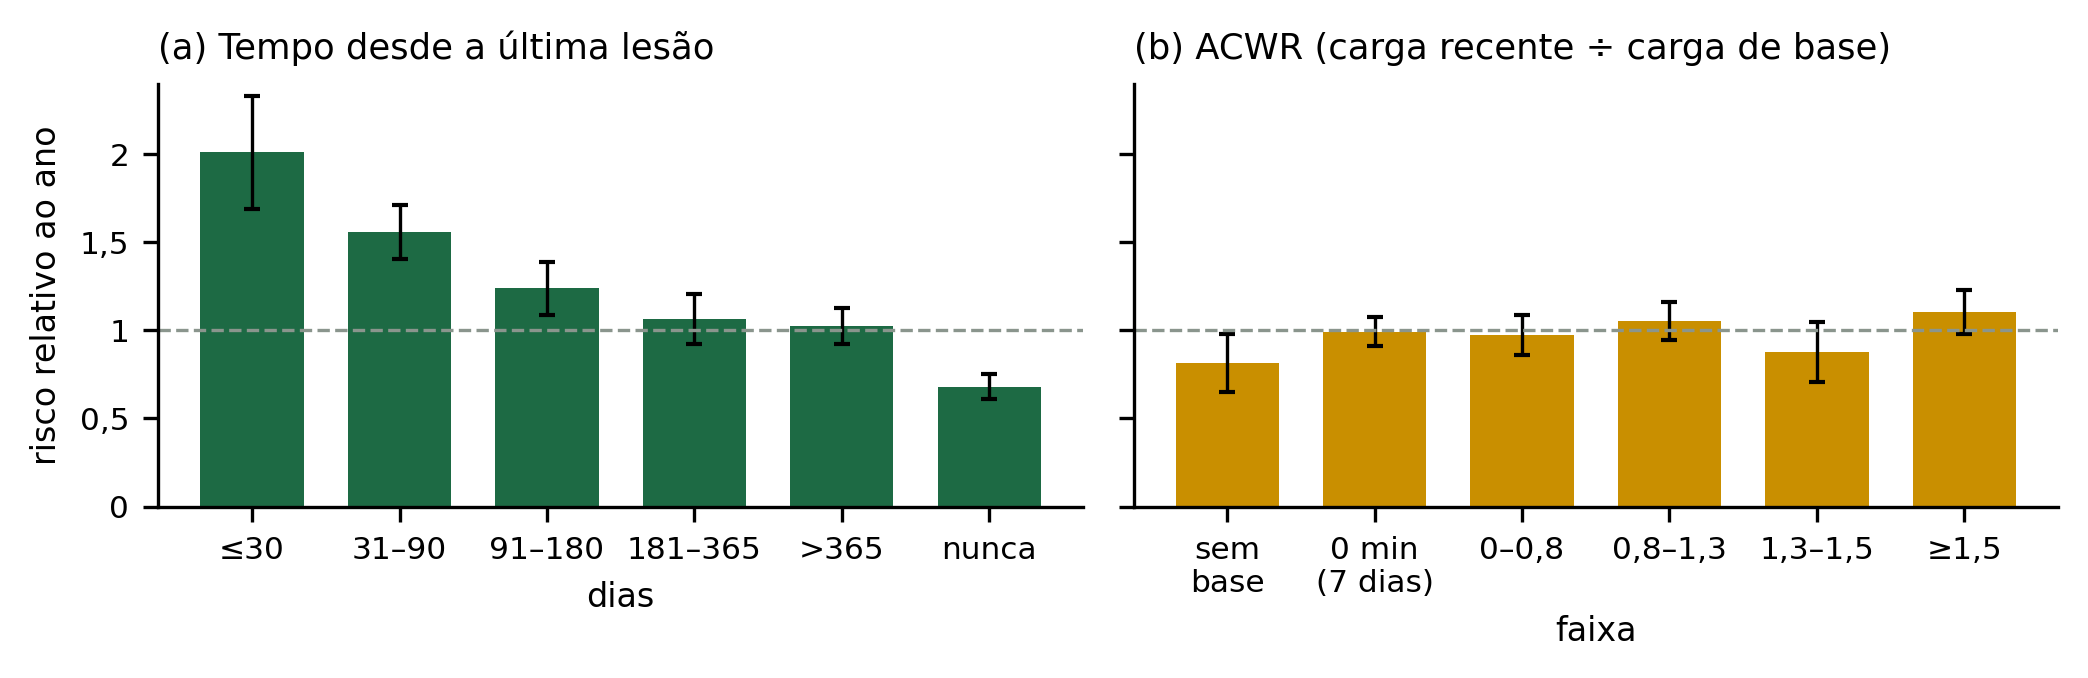
\includegraphics[width=\textwidth]{artigo_historico_vs_acwr.png}
\caption{Risco de lesão em 14 dias relativo à média do ano, com margem de erro de 95\%. (a) Por tempo desde a última lesão. (b) Por faixa de ACWR; ``sem base'' indica jogador sem minutos nas quatro semanas anteriores. A linha tracejada é o risco médio.}
\label{fig:eda}
\end{figure*}

\subsection{Comparação dos modelos}

A regra clássica da literatura, que considera em risco quem tem ACWR de $1{,}5$ ou mais, não foi melhor que o acaso. A regra simples mais eficaz foi dar mais risco a quem se lesionou há menos tempo. A Tabela~\ref{tab:modelos} compara essa regra com os quatro modelos.

\begin{table}[!t]
\caption{Desempenho no teste. AP com margem de erro (IC 95\%) e quantas vezes a taxa de lesões no grupo de 10\% de maior risco supera a média}
\label{tab:modelos}
\centering
\setlength{\tabcolsep}{4pt}
\begin{tabular}{llcccc}
\toprule
Corte & Modelo & AP & IC 95\% & AUC & Top 10\% \\
\midrule
A & Regra de recência & 0{,}095 & 0{,}080--0{,}114 & 0{,}588 & 1{,}77 \\
(acaso: & Reg. logística & \textbf{0{,}118} & 0{,}098--0{,}141 & 0{,}639 & 2{,}15 \\
0{,}069) & Random Forest & 0{,}108 & 0{,}092--0{,}129 & 0{,}618 & 1{,}88 \\
 & XGBoost & 0{,}111 & 0{,}094--0{,}133 & 0{,}620 & 2{,}13 \\
 & MLP & 0{,}067 & 0{,}060--0{,}078 & 0{,}501 & 0{,}89 \\
\midrule
B & Regra de recência & 0{,}117 & 0{,}099--0{,}138 & 0{,}604 & 1{,}45 \\
(acaso: & Reg. logística & \textbf{0{,}140} & 0{,}119--0{,}169 & 0{,}646 & 2{,}03 \\
0{,}084) & Random Forest & 0{,}126 & 0{,}110--0{,}148 & 0{,}639 & 1{,}76 \\
 & XGBoost & 0{,}127 & 0{,}109--0{,}152 & 0{,}633 & 1{,}79 \\
 & MLP & 0{,}098 & 0{,}087--0{,}114 & 0{,}557 & 1{,}30 \\
\midrule
C & Reg. logística & \textbf{0{,}139} & 0{,}118--0{,}168 & 0{,}652 & 2{,}00 \\
(acaso: & Random Forest & 0{,}127 & 0{,}110--0{,}150 & 0{,}630 & 1{,}85 \\
0{,}084) & XGBoost & 0{,}130 & 0{,}112--0{,}154 & 0{,}645 & 1{,}82 \\
 & MLP & 0{,}109 & 0{,}096--0{,}127 & 0{,}606 & 1{,}40 \\
\bottomrule
\end{tabular}
\end{table}

A regressão logística, o modelo mais simples, teve o melhor resultado nos três cortes. No corte B, $17\%$ dos jogos do grupo de $10\%$ de maior risco foram seguidos de lesão, contra $8{,}4\%$ na média, e esse grupo reuniu $20\%$ dos jogos seguidos de lesão. Contando lesões diferentes, ele alcançou $135$ das $525$ lesões do ano ($26\%$). A Figura~\ref{fig:decil} divide a lista de risco em dez partes iguais: a taxa de lesão cresce quase sem interrupção, de menos da metade da média nas duas partes de menor risco até o dobro na de maior risco.

\begin{figure}[!t]
\centering
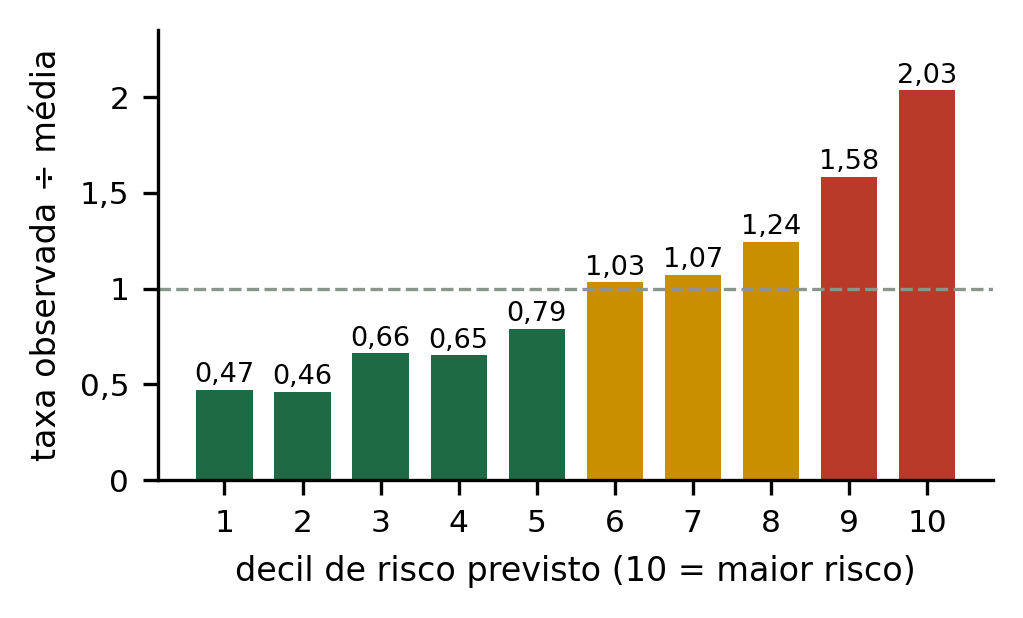
\includegraphics[width=\columnwidth]{artigo_lift_decil.png}
\caption{Taxa de lesão em cada décimo da lista de risco da regressão logística (treino em 2024, teste em 2025), dividida pela taxa média. A linha tracejada é a média.}
\label{fig:decil}
\end{figure}

A Tabela~\ref{tab:confusao} mostra o mesmo resultado como matriz de confusão, tratando como alerta os $10\%$ de jogos de maior risco. Dos $1{.}192$ alertas, $203$ foram seguidos de lesão, uma precisão de $17\%$. Dos $998$ jogos seguidos de lesão, $795$ ficaram fora da lista, então o recall foi de $20\%$. A Figura~\ref{fig:pr} mostra o que acontece com outros tamanhos de lista. A regressão logística fica acima dos outros modelos até capturar cerca de $40\%$ dos jogos seguidos de lesão; daí em diante as curvas se juntam. Uma lista maior pega mais lesões, mas a precisão cai para perto de $12\%$, pouco acima dos $8{,}4\%$ do acaso.

\begin{table}[!t]
\caption{Matriz de confusão da regressão logística no corte B (teste em 2025), com alerta para os 10\% de jogos de maior risco}
\label{tab:confusao}
\centering
\begin{tabular}{lrr}
\toprule
 & Lesão em 14 dias & Sem lesão \\
\midrule
Alerta & $203$ & $989$ \\
Sem alerta & $795$ & $9{.}934$ \\
\bottomrule
\end{tabular}
\end{table}

\begin{figure}[!t]
\centering
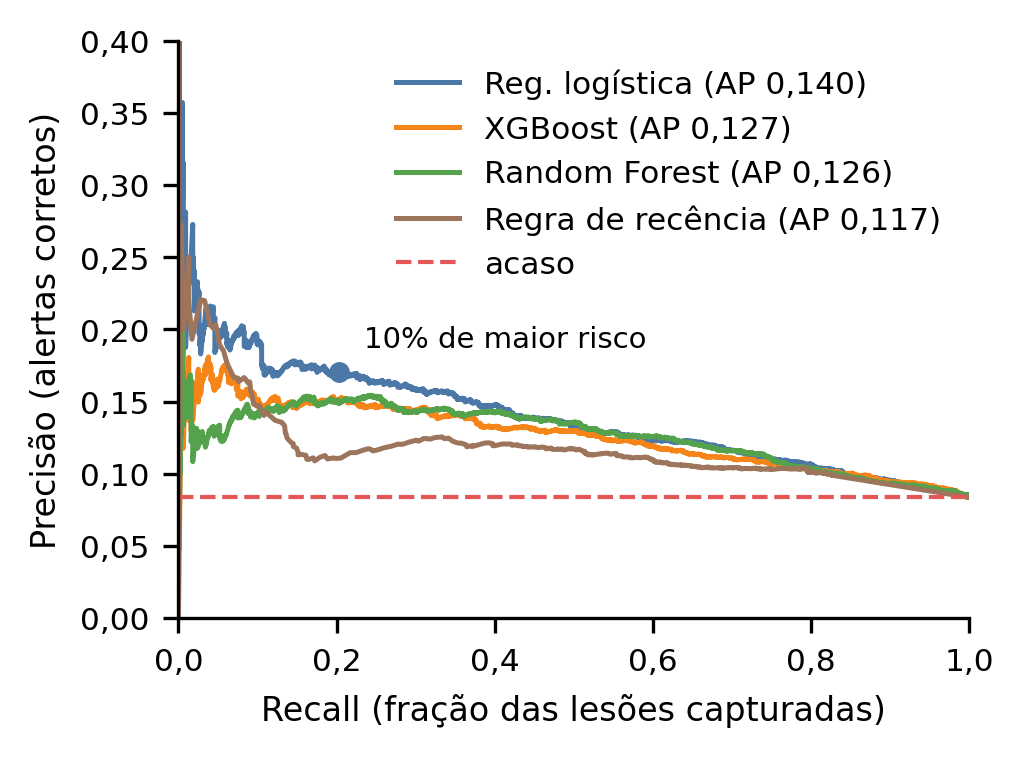
\includegraphics[width=\columnwidth]{artigo_curva_pr.png}
\caption{Curva de precisão e recall no corte B (treino em 2024, teste em 2025). Cada ponto de uma curva corresponde a um tamanho de lista de alerta. O ponto marcado é a lista com os 10\% de maior risco da regressão logística. A linha tracejada é o acaso.}
\label{fig:pr}
\end{figure}

Random Forest e XGBoost ficaram próximos, com margens de erro que se sobrepõem às da regressão logística. A rede neural foi a pior e, no corte A, não superou o acaso. Usar todos os anos anteriores no treino (corte C) não melhorou o resultado de usar só 2024. O primeiro critério foi atendido.

\subsection{Sobreajuste e variação entre execuções}

A Tabela~\ref{tab:ajuste} compara a AUC no treino, na validação cruzada e no teste do corte B. A regressão logística tem quase o mesmo valor nas três situações ($0{,}68$, $0{,}65$ e $0{,}65$), sinal de que não decorou o treino. O Random Forest chega a $0{,}81$ no próprio treino e cai para $0{,}62$ a $0{,}64$ fora dele. As árvores memorizam parte do treino. Com folha mínima de $25$ jogos, a AUC no treino chega a $0{,}97$ e a do teste cai para $0{,}625$; a folha de $100$, escolhida pela validação cruzada, limita essa memorização. O XGBoost fica entre os dois. Os cortes A e C mostram o mesmo padrão, com o Random Forest em $0{,}92$ e $0{,}85$ no treino.

\begin{table}[!t]
\caption{AUC no treino, na validação cruzada (média $\pm$ desvio-padrão das cinco partes) e no teste, corte B}
\label{tab:ajuste}
\centering
\begin{tabular}{lccc}
\toprule
Modelo & Treino & Validação cruzada & Teste \\
\midrule
Reg. logística & $0{,}676$ & $0{,}650 \pm 0{,}022$ & $0{,}646$ \\
Random Forest & $0{,}814$ & $0{,}620 \pm 0{,}021$ & $0{,}639$ \\
XGBoost & $0{,}743$ & $0{,}629 \pm 0{,}022$ & $0{,}633$ \\
MLP (1 inicialização) & $0{,}500$ & $0{,}529 \pm 0{,}034$ & $0{,}504$ \\
\bottomrule
\end{tabular}
\end{table}

O desvio-padrão entre as partes da validação cruzada ficou entre $0{,}02$ e $0{,}04$ de AUC nos três cortes. Isso é maior que a distância entre regressão logística, Random Forest e XGBoost no teste, o que confirma o empate entre os três. A rede neural é instável. Com uma só inicialização, a AUC fica perto de $0{,}5$ nos cortes A e B. Entre as $10$ inicializações, a AP no teste do corte B foi de $0{,}093 \pm 0{,}006$. A média das $10$ previsões, usada na Tabela~\ref{tab:modelos}, chegou a $0{,}098$ e continuou sendo a pior dos quatro modelos.

\subsection{O que cada grupo de atributos acrescenta}

A Figura~\ref{fig:ablacao} mostra o desempenho com cada combinação de atributos. Só com o perfil do jogador, os modelos ficam perto do acaso. O histórico de lesões traz o maior ganho, e o calendário acrescenta mais um pouco. A carga de minutos, sozinha, não supera o acaso.

\begin{figure*}[!t]
\centering
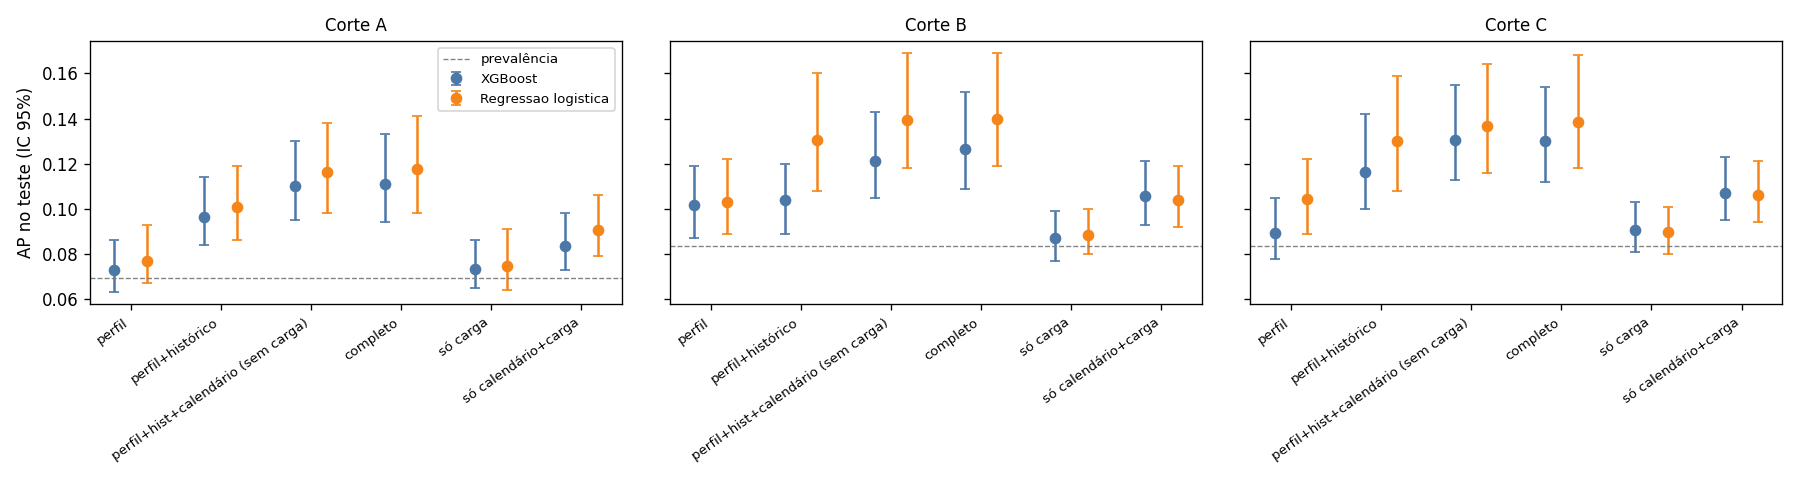
\includegraphics[width=\textwidth]{m03_ablacao.png}
\caption{AP no teste para cada combinação de atributos, com margem de erro de 95\%. A linha tracejada indica o acaso.}
\label{fig:ablacao}
\end{figure*}

A Tabela~\ref{tab:delta} mostra quanto a AP muda quando a carga é acrescentada aos demais atributos. Em cinco das seis comparações, a diferença pode ser zero. A exceção é o XGBoost no corte B, com ganho de $0{,}006$. Pela regra definida antes, isso basta para atender ao segundo critério. O efeito, porém, é frágil: é pequeno, desaparece no corte C, que usa os mesmos dados de teste, e não aparece na regressão logística. Além disso, o XGBoost com carga continua abaixo da regressão logística sem carga.

\begin{table}[!t]
\caption{Variação da AP ao acrescentar a carga de minutos, com margem de erro de 95\%}
\label{tab:delta}
\centering
\begin{tabular}{llr}
\toprule
Corte & Modelo & Variação da AP (IC 95\%) \\
\midrule
A & Reg. logística & $+0{,}0017$ ($-0{,}0003$ a $+0{,}0039$) \\
A & XGBoost & $+0{,}0006$ ($-0{,}0048$ a $+0{,}0064$) \\
B & Reg. logística & $+0{,}0004$ ($-0{,}0036$ a $+0{,}0043$) \\
B & XGBoost & $+0{,}0057$ ($+0{,}0006$ a $+0{,}0119$) \\
C & Reg. logística & $+0{,}0019$ ($-0{,}0009$ a $+0{,}0046$) \\
C & XGBoost & $-0{,}0007$ ($-0{,}0043$ a $+0{,}0027$) \\
\bottomrule
\end{tabular}
\end{table}

\subsection{Testes de robustez}
\label{sec:robustez}

Os resultados se mantiveram em cinco verificações (Tabela~\ref{tab:robustez}). Nos anos de registro mais pobre (treino em 2022, teste em 2023), os modelos continuaram melhores que o acaso. Incluir as lesões do dia do jogo quase não mudou a AP. Na validação cruzada de 2024--25, deixar clubes inteiros fora do treino deu a mesma AP que deixar jogadores fora, o que mostra que o modelo funciona para clubes que não viu. Jogadores que nunca apareceram no treino tiveram previsões tão boas quanto os demais. Por fim, pesos de classe e redução da classe negativa não mudaram a AP do XGBoost; só distorceram as probabilidades, que passaram a superestimar o risco: a média do risco previsto, que deveria ficar perto dos $8{,}4\%$ reais, subiu de $0{,}07$ para até $0{,}45$.

\begin{table}[!t]
\caption{AP nos testes de robustez. Regressão logística, salvo indicação}
\label{tab:robustez}
\centering
\footnotesize
\setlength{\tabcolsep}{3pt}
\begin{tabular}{>{\raggedright\arraybackslash}p{0.42\columnwidth} >{\raggedright\arraybackslash}p{0.2\columnwidth} >{\raggedright\arraybackslash}p{0.3\columnwidth}}
\toprule
Verificação & AP & Referência \\
\midrule
Treino 2022, teste 2023 & $0{,}030$ & acaso: $0{,}020$ \\
Incluindo lesões do dia do jogo (corte B) & $0{,}147$ & alvo principal: $0{,}140$ \\
Clubes fora do treino (2024 / 2025) & $0{,}124$ / $0{,}139$ & jogadores fora: $0{,}120$ / $0{,}143$ \\
Jogadores nunca vistos no treino (corte B) & $0{,}147$ & já vistos: $0{,}139$ \\
XGBoost sem peso, com pesos ou com redução de negativos (corte B) & $0{,}126$ a $0{,}127$ & média do risco previsto: $0{,}07$ a $0{,}45$ \\
\bottomrule
\end{tabular}
\end{table}

\subsection{Interpretação}

Embaralhar o histórico de lesões reduz a AP em $19\%$ a $31\%$; o calendário, em $15\%$ a $17\%$; o perfil, em $3\%$ a $9\%$; a carga, em no máximo $5\%$. Na análise SHAP do XGBoost (Figura~\ref{fig:shap}), o atributo de maior peso foi o número de jogos do clube nos $14$ dias seguintes: sem jogos à frente, o risco previsto cai bastante. Em seguida vêm o tempo desde a última lesão, a duração dela e o número de lesões anteriores. Ser goleiro reduz o risco. A carga aparece no SHAP com mais peso do que na primeira análise, porque o modelo a usa, mas, quando ela é retirada, compensa com o calendário e o histórico, que carregam a mesma informação.

\begin{figure}[!t]
\centering
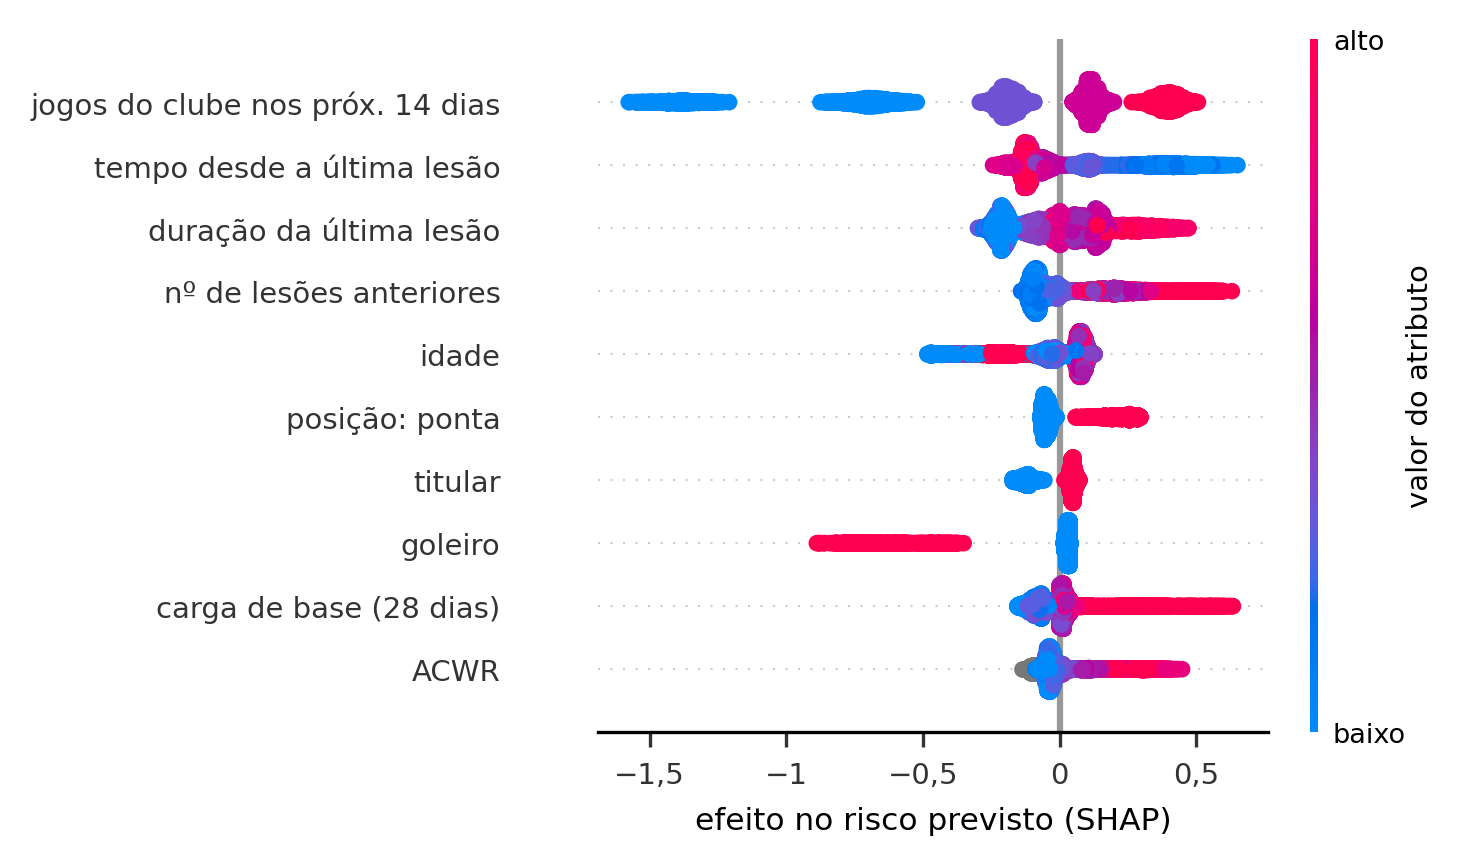
\includegraphics[width=\columnwidth]{artigo_shap.png}
\caption{SHAP do XGBoost no teste de 2025, para os dez atributos de maior peso. Cada ponto é um jogo. A posição horizontal mostra quanto o atributo aumentou (direita) ou reduziu (esquerda) o risco previsto; a cor indica o valor do atributo naquele jogo.}
\label{fig:shap}
\end{figure}

\subsection{Discussão}

Dados públicos permitem ordenar o risco de lesão melhor do que o acaso, de forma modesta e estável. A AUC de $0{,}65$ está na faixa obtida por Chang \textit{et al.}~\cite{chang2024} com dados públicos e abaixo dos $0{,}74$ de Huth \textit{et al.}~\cite{huth2026} com GPS. Essas comparações são aproximadas, porque cada estudo usa outra liga, outra definição de lesão e outra divisão dos dados. A divisão aleatória de Chang \textit{et al.} mistura temporadas e tende a dar números mais altos que a divisão no tempo usada aqui. Na prática, o grupo de maior risco apontado pelo modelo tem o dobro da taxa média de lesões, e esse resultado se repetiu em todos os testes.

O sinal vem de duas fontes. A primeira é o histórico: quem se lesionou recentemente tem mais chance de se lesionar de novo, como também observaram Majumdar \textit{et al.}~\cite{majumdar2024}. A segunda é a exposição: quem tem mais jogos pela frente tem mais oportunidades de se lesionar.

A carga de minutos acrescentou pouco ou nada, e a regra clássica da ACWR não superou o acaso. Os estudos que associam a ACWR a lesões medem a carga de treino com GPS. Minutos em jogos oficiais são uma parte pequena do esforço do atleta, que inclui treinos, viagens e recuperação. Nesta base, quem joga mais minutos se lesiona um pouco mais porque continua jogando, e não necessariamente por excesso de esforço.

Modelos simples bastaram. A regressão logística empatou ou superou as árvores, como em parte dos estudos revisados por Leckey \textit{et al.}~\cite{leckey2025}, e a rede neural ficou por último. Com algumas centenas de lesões no treino, há pouco padrão complexo a aprender. Corrigir o desbalanceamento das classes também não ajudou, o que sugere que o ganho relatado por Tonizzo~\cite{tonizzo2025} com essas técnicas pode vir só de uma mudança no ponto de corte.

A mudança no registro do Transfermarkt vale para qualquer estudo com essa fonte. A taxa de lesões triplicou sem mudança real aparente, de forma desigual entre clubes. Isso pode explicar, em parte, por que o clube aparece como preditor forte em Chang \textit{et al.}~\cite{chang2024}.

\section{Conclusões, Limitações da Abordagem e Trabalhos Futuros}

\subsection{Síntese das contribuições}

Este trabalho perguntou se dados públicos bastam para estimar o risco de lesão de jogadores profissionais. Para responder, montamos uma base com quatro temporadas da Série~A (2022 a 2025), verificamos a qualidade dos registros do Transfermarkt e comparamos quatro modelos de aprendizado de máquina contra regras simples. A resposta é sim, com um alcance limitado. Treinado em 2024 e testado em 2025, o melhor modelo, uma regressão logística, chegou a uma AUC de $0{,}65$, e os $10\%$ de jogos que ele apontou como mais arriscados tiveram o dobro da taxa média de lesões. O critério de utilidade definido antes dos testes foi atendido, e o resultado se repetiu nos testes de robustez.

O sinal útil veio quase todo de duas fontes: o histórico de lesões do jogador e o número de jogos que o clube tem pela frente. A carga de minutos, base da ideia que motivou o trabalho, acrescentou pouco. Seu ganho só foi claro em uma de seis comparações, e a regra clássica da ACWR não superou o acaso. Com dados públicos, portanto, o melhor indicador de risco é o passado de lesões do atleta. Minutos em jogos oficiais não substituem a medição de carga feita com GPS nos treinos. Também não foi preciso um modelo complexo: a regressão logística empatou ou superou as árvores e a rede neural.

A segunda contribuição é um alerta sobre a fonte. A taxa de lesões registrada no Transfermarkt triplicou a partir de 2024, em todas as faixas de gravidade e de forma desigual entre clubes, sem sinal de aumento real. Quem usar essa base para estudar lesões precisa medir essa mudança antes de comparar anos ou clubes, e deve treinar e testar o modelo em períodos de registro parecido.

Na prática, o modelo serve para ordenar o elenco e chamar a atenção da equipe médica para quem merece acompanhamento mais de perto. Ele não substitui a avaliação clínica, já que só $17\%$ dos alertas viraram lesão, e a decisão sobre escalar um atleta continua com a equipe médica.

\subsection{Limitações}

A maior limitação está na fonte. O alvo é o que o Transfermarkt registra, e esse registro mudou a partir de 2024, mais em alguns clubes do que em outros. Lesões leves e pouco divulgadas podem estar ausentes, sobretudo em 2022 e 2023. Não existe fonte oficial com a qual conferir os registros.

A amostra real é pequena. Os $2{.}367$ casos positivos vêm de $1{.}212$ lesões, e o treino do corte principal, só com 2024, tem $416$. Por isso testamos poucas configurações de cada modelo, e modelos mais flexíveis, como a rede neural, ficaram instáveis.

A generalização foi testada de forma limitada. Usamos uma única liga, e as observações são só jogos da Série~A, então jogadores que atuam pouco nela ficam de fora. O corte principal tem um único ano de teste, 2025, e não houve validação em outra base.

Os atributos medem pouco do esforço real. Sem dados de treino, GPS, viagens ou sono, a carga se resume aos minutos em jogos oficiais. O número de jogos do clube nos $14$ dias seguintes mede exposição, e não esforço do atleta.

Há ainda limites no desenho e no desempenho. A janela de $14$ dias faz uma mesma lesão aparecer em vários jogos, e a data registrada da lesão às vezes cai no dia seguinte ao jogo. A AUC de $0{,}65$ e a precisão de $17\%$ significam que cinco de cada seis alertas são falsos. As probabilidades não foram calibradas: com peso de classe, a regressão logística do corte B superestima o risco, e a saída deve ser lida como ordem de prioridade, e não como chance real de lesão. Por fim, a coleta precisa respeitar um intervalo entre acessos ao site, o que limitou a base a uma liga.

\subsection{Trabalhos futuros}

Cada limitação aponta um próximo passo. Para separar mudança de registro e mudança real, os registros do Transfermarkt podem ser cruzados com boletins médicos dos clubes e com a imprensa esportiva em uma amostra de clubes. Para ampliar a base, os mesmos scripts podem coletar a Série~B, as copas nacionais e ligas de outros países. Com isso, seria possível treinar no Brasil e testar em outra liga, como validação externa, e repetir o teste em 2026 para saber se o registro se estabilizou.

Novos atributos públicos podem medir melhor o esforço: distância e tempo de viagem entre as cidades dos jogos, tipo de gramado e eventos de jogo, como faltas sofridas. Do lado dos modelos, sugerimos calibrar as probabilidades, escolher o tamanho da lista de alerta junto com uma equipe médica e testar modelos de tempo até a lesão, que tratam a repetição dos casos positivos sem a janela fixa de $14$ dias. Com uma base maior, vale também uma busca mais ampla de hiperparâmetros.


\begin{thebibliography}{00}

\bibitem{gabbett2016}
T.~J. Gabbett, ``The training--injury prevention paradox: should athletes be training smarter and harder?'' \textit{Br. J. Sports Med.}, vol.~50, no.~5, pp.~273--280, 2016, \doilink{10.1136/bjsports-2015-095788}.

\bibitem{majumdar2022}
A.~Majumdar, R.~Bakirov, D.~Hodges, S.~Scott, and T.~Rees, ``Machine learning for understanding and predicting injuries in football,'' \textit{Sports Med. Open}, vol.~8, Art.~no.~73, 2022, \doilink{10.1186/s40798-022-00465-4}.

\bibitem{saberisani2025}
R.~Saberisani \textit{et al.}, ``Prediction of football injuries using GPS-based data in Iranian professional football players: a machine learning approach,'' \textit{Front. Sports Act. Living}, vol.~7, Art.~no.~1425180, 2025, \doilink{10.3389/fspor.2025.1425180}.

\bibitem{huth2026}
M.~Huth \textit{et al.}, ``Injury prediction in elite women's football: an integrative machine learning-based decision-support framework,'' \textit{npj Digit. Med.}, Jul.~2026, \doilink{10.1038/s41746-026-02937-3}.

\bibitem{leckey2025}
C.~Leckey, N.~van Dyk, C.~Doherty, A.~Lawlor, and E.~Delahunt, ``Machine learning approaches to injury risk prediction in sport: a scoping review with evidence synthesis,'' \textit{Br. J. Sports Med.}, vol.~59, no.~7, pp.~491--500, 2025, \doilink{10.1136/bjsports-2024-108576}.

\bibitem{page2023}
R.~M. Page, A.~Field, B.~Langley, L.~D. Harper, and R.~Julian, ``The effects of fixture congestion on injury in professional male soccer: a systematic review,'' \textit{Sports Med.}, vol.~53, no.~3, pp.~667--685, 2023, \doilink{10.1007/s40279-022-01799-5}.

\bibitem{jaja2026}
D.~Jaja, ``Building an injury risk model with football data,'' Sportmonks, Jul.~2, 2026. [Online]. Available: \url{https://www.sportmonks.com/blogs/building-an-injury-risk-model-with-football-data/}. Accessed: Oct.~10, 2026.

\bibitem{rossi2018}
A.~Rossi, L.~Pappalardo, P.~Cintia, F.~M. Iaia, J.~Fernàndez, and D.~Medina, ``Effective injury forecasting in soccer with GPS training data and machine learning,'' \textit{PLoS ONE}, vol.~13, no.~7, Art.~no.~e0201264, 2018, \doilink{10.1371/journal.pone.0201264}.

\bibitem{majumdar2024}
A.~Majumdar, R.~Bakirov, D.~Hodges, S.~McCullagh, and T.~Rees, ``A multi-season machine learning approach to examine the training load and injury relationship in professional soccer,'' \textit{J. Sports Anal.}, vol.~10, no.~1, pp.~47--65, 2024, \doilink{10.3233/JSA-240718}.

\bibitem{chang2024}
V.~Chang, S.~Sajeev, Q.~A. Xu, M.~Tan, and H.~Wang, ``Football analytics: assessing the correlation between workload, injury and performance of football players in the English Premier League,'' \textit{Appl. Sci.}, vol.~14, no.~16, Art.~no.~7217, 2024, \doilink{10.3390/app14167217}.

\bibitem{everett2024}
G.~Everett, R.~Beal, T.~Matthews, T.~J. Norman, and S.~D. Ramchurn, ``The strain of success: a predictive model for injury risk mitigation and team success in soccer,'' arXiv:2402.04898, 2024.

\bibitem{tonizzo2025}
G.~Tonizzo, ``Predictive models for injury prevention in football: a machine learning approach using performance and injury data,'' M.S. thesis, Politecnico di Torino, Turin, Italy, 2025.

\bibitem{lundberg2017}
S.~M. Lundberg and S.-I. Lee, ``A unified approach to interpreting model predictions,'' in \textit{Proc. 31st Int. Conf. Neural Inf. Process. Syst. (NeurIPS)}, Long Beach, CA, USA, 2017, pp.~4765--4774.

\bibitem{williams2017}
S.~Williams, S.~West, M.~J. Cross, and K.~A. Stokes, ``Better way to determine the acute:chronic workload ratio?'' \textit{Br. J. Sports Med.}, vol.~51, no.~3, pp.~209--210, 2017, \doilink{10.1136/bjsports-2016-096589}.

\bibitem{vandengoorbergh2022}
R.~van den Goorbergh, M.~van Smeden, D.~Timmerman, and B.~Van Calster, ``The harm of class imbalance corrections for risk prediction models: illustration and simulation using logistic regression,'' \textit{J. Am. Med. Inform. Assoc.}, vol.~29, no.~9, pp.~1525--1534, 2022, \doilink{10.1093/jamia/ocac093}.

\end{thebibliography}

\end{document}
